In the first sections of this chapter we outline the background, purpose and
objectives and the last section describes the scope of our research. Chapter 2
contains the theory needed for understanding the thesis, existing software and
some verification methods described in the standards. Methods is described in
Chapter 3 and the results in Chapter 4. In Chapter 5 and 6 we have a discussion
and some conclusions about the results.

%Background to the assignment. Why is it relevant?
\section{Background}
\subsection{The Development within Automotive Industry}
In the recent decades there has been a dramatic growth of information and
communications innovations within the automotive industry
\cite{CRC:embedded_handbook}. Analog vehicles have been transformed into complex
electromechanical systems \cite{Cambridge:controlsystems}. New features are
implemented (for example due to user demands, traffic safety or environmental
regulations \cite{Springer:advanced_microsystems}) requiring more computational
power and less energy consumption \cite{Springer:advanced_microsystems}.
The average car has already 80 ECUs (electronic computation units)
\cite{Springer:advanced_microsystems} and to deal with (integrate?) the extra
functionality, each ECU will (also?) need to become more complex
\cite{Springer:advanced_microsystems}. (F\"{o}rklara mer ing{\aa}ende att ECU
blir mer komplex pga man typ inte kan l\"{a}gga in fler ECUs i bilar f\"{o}r
d{\aa} \"{o}kar energianv\"{a}ndningen mer \"{a}n om man fixar b\"{a}ttre
ECUer \cite{Springer:advanced_microsystems}.)

\subsection{Extent of software in modern Vehicles}
(To picture how large part IT is of a new car:)
Developing a new car model costs up to one billion \euro
\cite{Clemens:tech_acceptance}, where electronics has reached a mean share of
one third of the value, divided 20\% sensor value, 40\% hardware value and 40\%
software value \cite{Wiley:internetworking}. The share of software has been
doubled the last 10 years \cite{Wiley:internetworking}.

More and more functions will be implemented; Intelligent traffic systems which
make the automotive vehicles communicate with the roadside management systems
\cite{Cambridge:controlsystems}, infotainment systems will bring, among other,
weather information through internet and emergency call support
\cite{Wiley:internetworking}\cite{Springer:advanced_microsystems}, traffic sign
recognition \cite{Springer:advanced_microsystems}, night vision
\cite{Wiley:internetworking}\cite{Springer:advanced_microsystems} and automated
parking \cite{Springer:advanced_microsystems}.

The number of lines of code running in a vehicle is another example of how
complex the automotive software is. The software running on a F-22 Raptor
and the F-35 Strike Fighter, US air force attack planes, has about 1.7 million
lines of code and 5.7 million lines of code respectively
\cite{IEEESpectrum:car_code}. The passenger plane Boeing 787 Dreamliner runs on
6.5 million lines of code where the average premium-class car has close to 100
million lines of code \cite{IEEESpectrum:car_code}.

\subsection{Introduction of standards}
Because of the high development costs, and the complexity of modern cars, car
manufacturers, suppliers and other companies related to the automotive industry
joined efforts in 2003 and created AUTOSAR, short for Automotive open system
architecture \cite{AUTOSAR:basic_info}. The main id\'{e} is to make it possible
for car manufacturers to buy independent components from different software
suppliers; the AUTOSAR motto is ``Cooperate on standards, compete on
implementation'' \cite{AUTOSAR:basic_info}.

Functional safety is introduced to the automotive industry with ISO 26262 in
late 2011\cite{ISO26262}. ISO 26262 named ``Road vehicles -- Functional safety''
is a general standard on how the development of vehicles should be made from
scratch to finish.

\subsection{Testing}
Functional safety demands testing (k\"{a}lla: bara att se p{\aa} iso 26262), and
testing accounts for around half of all software development costs
\cite{QUICKCHECK:lightweight}\cite{QUICKCHECK:software}. (the most common way to
test is unit testing.) reduce the cost is motivated and can be done by
automating the test generation process
\cite{QUICKCHECK:software}\cite{Testing:black_box}.














%Background to the assignment. Why is it relevant?
\section{Background-old}
The last decade of the 20th century resulted in a dramatic growth of technology
\cite{AUTOSAR:gilberg}. The rate is still increasing with up to 90\% of all
innovations being realized through electronics in the beginning of the 21st
century \cite{Frost_Sullivan:flyer}, and over 80 \% of all innovations in the
automotive industry are in the electronics and software area
\cite{SAFE:interoperability}.
%% eventuellt dela upp paragrafen h�r d� det �r tv� olika ideer; en om att
%% teknologin utvecklas snabbt och mycket, och en som handlar om att just bilar
%% blir mer komplexa.
The software-based systems in motor vehicles have become more complex, and are
moving toward handling more critical functions \cite{SAFE:interoperability}.
Vehicles have already begun to communicate with each other \cite{VOLVO:convoys},
and it is soon expected that roadside traffic management systems will also
interact with the systems in vehicles \cite{SURVEY:car_communications}.

While the systems become more complex the software must be fault-tolerant and
safe. Testing, validation and verification is a need and should follow all
product development phases, from start to finish. The problem is that testing
is %% introducerar "product development phases" utan f�rklaring. beh�vs den?
both time consuming and labour intensive, accounting for up to 50 \% of the
development cost \cite{QUICKCHECK:lightweight}. Unit tests adds additional
complexity to the code. It is very important to test and verify all steps of the
development.

The complexity issue is that in systems such as microprocessors the number of
possible failure states is so large that it is considered
infinite \cite{COURSEBOOK:safety-critical}. This makes it impossible exhaustively
test the system, and therefore, also make the detection of failures unreliable.

Quviq QuickCheck has the ability to automate this process, and allow the
developer to write properties instead of tests. These properties makes it
possible for QuickCheck to create arbitrary input vectors that can be feed to
the code. Figure~\ref{IMG:phase_model} shows the different steps of the software
development process and the test and verification phases it has.

\begin{figure}[!ht]
  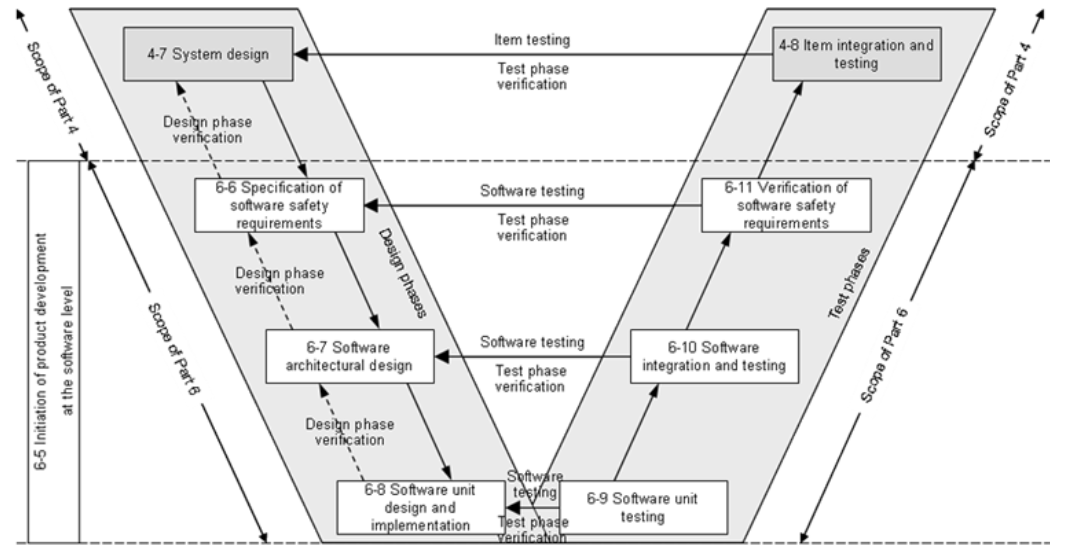
\includegraphics[keepaspectratio, width=\linewidth]{pictures/V}
  \label{IMG:phase_model}
  \caption{Phase model for software development}
\end{figure}

The first step is the system design. At this point the system specification is
written, and then the software specifications. When all specifications exists,
the next phase is to design the software architecture. The last part of the
design is software unit design and implementation. All phases must be a
verification of the former phase.

When the implementation is done, it is time for the test phases. These begins
with software unit testing which tests the software unit design phase. If the
tests verifies that the software unit design and implementation is correct, the
test phase moves on to the architectural design and then to verification of
software safety requirements.
The last test phase verifies that the system is
designed according to the specification. %It is important that the test phases
%test the specifications and not the
%implementation.

Because all manufacturers strive for the lowest production cost, car
manufacturers together with suppliers and other related companies, from the
automotive industry, have come to agree over a standard for the software
architecture in automotive vehicles. This standard is named AUTOSAR (AUTomotive
Open System ARchitecture) and makes it possible to select different suppliers
for different modules of the system.

AUTOSAR is very complex and since it is quite new, it still suffers from child
deceases, with requirements that are confusing and contradictorily. The first
versions of AUTOSAR is made without functional safety in mind.

%Aim for the work. What should be accomplished?
\section{Purpose}
The purpose is to automate the testing process in an effective and good way.
To make it possible to raise the Automotive Safety Integration Level (ASIL), in
the software unit design and implementation phase and in the software %% n�mner
 %% ASIL utan att ha pratat om det tidigare.
architectural design phase, a check must be done to see if it exist a tool that
can be used in order to perform a semi formal verification of a module, and
then make this process generalized for modules in coexistence.\\ %% v�ldigt l�ng
 %% mening

The purpose is also to be able to decrease the number of needed unit tests in
the software unit design and implementation phase. Even further is the goal to
introduce semi formal verification of the software architectural design phase.
The functional safety concept will be most important in this phase.

%question formulation?
%The problem at hand, the assignment
\section{Objective}
The first problem at hand is to evaluate what ``semi formal verification'',
according to the ISO-standard, means. In formal methods of mathematics, formal
verification means to prove the correctness of algorithms.
The ISO-standard mentions both ``formal verification'' and ``semi
formal verification'' for software development, but does not describe how to
achieve any of these.
This evaluation must be done to get knowledge of how to properly implement
functional safety and reach an ASIL classification, using automated testing.

%The second problem is to evaluate if QuickCheck can be used to achieve this.
%QuickCheck grants the ability to automate the testing, and knowledge of this
%ool exist in the corporation where this thesis is done. %% F�retaget hm....

A model for an AUTOSAR module needs to be implemented. For this to be a good
model some questions first needs to be answered.
How can one achieve good test cases for the model? How can one tweak the test
generation to find test cases that are interesting in a safety critical point of
view? Is the implemented model together with the generated tests good enough to
reach the goals?

The test generation is a big problem when verifying a model. With unit tests, one
can argue for that each line of code has been executed (100\% code coverage),
but that is just a statement for that everything has been executed. Have it been
executed correctly?
Are every combination of computations in the system necessary to ensure
correctness, or with other words, is it possible to collapse some states in the
system's state space without endangering the safety of the hole system?

After the model has been implemented, there must be an evaluation of the
solution. Does it ensure functional safety? How can one measure the
size of the state space that is actually verified?
Even if test generation has been done properly, the solution might not be within
the ISO-standards means of functional safety.

One must propose and motivate what should be done to be able to
achieve a semi formal verification. This can include a confidence interval
for how certain the verification is. The confidence interval would help
describing the visited state space because it is probably not feasible to
exhaustively visit all states due to the state space explosion problem.

The main objective is to prove that it is possible to do semi formal
verification for an AUTOSAR module and its specification.
It should not matter which configuration that is active and even further
how the module is implemented, because the specification should hold for all
configurations and implementations. This gives rise to that every company that
implements the module should be able to run the final code to achieve ``semi
formal verification''. Since modules in AUTOSAR are dependent the work presented here
should be generalized so it can be hooked on when implementing test suits,
using the same techniques, for other modules.

%Limitations. What should be left out and why?
\section{Scope}
We will use AUTOSAR 4.0 revision 3 for our thesis work.
Since this version of AUTOSAR consists of around 80 specifications and other
auxiliary materials\cite{AUTOSAR:URL}, we will limit our scope to one
specification. The module of this thesis is the WatchdogManager. This
module provides monitoring services used to maintain correctness. This
module is chosen because it got dependencies, is used to report
development and production errors, but mainly because it executes
safety-critical work.

Also the aim of the work is to verify software components. In other words no
work considered hardware or a combination of hardware and software will be
prioritized. All implemented code for the verification will run on a standard
PC-machine.

%% l�gga till ett stycke ang�ende att vi bara g�r in p� 6-9 och 6-10, och inte
%% p� 6-8 eller 6-11.
